%=================================================================================================%
% This is a template designed for Chin. Phys. B (Dated 12 November 2014)
% Only one step to compile: PDFTeXify
%=================================================================================================%
\documentclass{cpbtex}

\begin{document}
\begin{CJK*}{GBK}{song}

\title{Manuscript title}

% Title should be concise; avoid abbreviations if possible; and not begin with `A', `An', `The', or `Study on'.

\author{First Author$^{1}$, \ Second Author$^{2}$, $\ldots$, \ and \ Last Author$^{2,3,}$\thanks{Corresponding author. E-mail:~xxx@xxx.edu}\\
$^{1}${First affiliation}\\  % The line break was forced via \\
$^{2}${Second affiliation}\\ % The line break was forced via \\
$^{3}${Third affiliation}}   % The line break was forced via \\

% 1. For Chinese authors, the name in Chinese characters should also be given. For example, Gang Liu(����), Xiao-Ming Li(������)
% 2. Please ensure that every author approves the submission of the manuscript
% 3. Abbreviations should not be used in the affiliations

\date{\today}
\maketitle

\begin{abstract}
The abstract is a concise (short and clear) summary of your work. It should clearly state the problem, the methods used, the main results, and the conclusions, and should not include citations and formulas.
\end{abstract}

\textbf{Keywords:} %no more than four sets of keywords should be provided

\textbf{PACS:} %no more than four PACS codes should be provided: check https://cpb.iphy.ac.cn/UserFiles/File/PACS2010Regular-Edition.pdf


\section{Introduction}
This template is recommended for authors who will submit their manuscript in LaTex to Chinese Physics B.\ucite{1} You are also advised to read some articles (Refs.~\cite{2,3,4,5,6}) already published in the journal. It can be very helpful for preparing your own manuscript, especially for preparing formatted formulas, tables, figures, and references.

Note: A brief guidance on how to prepare a manuscript is also given at the end of this template (after the Reference section).

\section{First-level heading (e.g., Theoretical method or Experimental setup)}


\section{First-level heading (e.g., Results and discussion)}


\subsection{Second-level heading}


\subsubsection{Third-level heading}


\subsection{Second-level heading}


\subsubsection{Third-level heading}


\section{Conclusion}


\addcontentsline{toc}{chapter}{Appendix A: Appendix section heading}
\section*{Appendix A: Appendix heading}
Appendix is optional.



\section*{Data availability statement}
The data that support the findings of this study are openly available in Science Data Bank at\\ https://www.doi.org/XXXXXXX. This statement should be given if some related data have been deposited in \href{https://www.scidb.cn/en}{Science Data Bank}.

\addcontentsline{toc}{chapter}{Acknowledgment}
\section*{Acknowledgment}
Financial supports are given here. The scientific contributions from other people or groups are also acknowledged here.




\addcontentsline{toc}{chapter}{References}
\begin{thebibliography}{99}\footnotesize
\itemsep=-3pt plus.2pt minus.2pt   % set the reference line spacing
\bibitem{1} \href{https://cpb.iphy.ac.cn/EN/column/column32.shtml}{https://cpb.iphy.ac.cn/EN/column/column32.shtml}


\bibitem{2}  Zheng M T, Schwier E F, Iwasawa H and Shimada K \href{https://doi.org/10.1088/1674-1056/ab9196}{2020 \emph{Chin. Phys. B} \textbf{29} 067901}

\bibitem{3} Zeng H L and Aurell E \href{https://doi.org/10.1088/1674-1056/ab8da6}{2020 \emph{Chin. Phys. B} \textbf{29} 080201}

\bibitem{4} Zhao R T, Xing B Y, Mu H M, Fu Y H and Zhang L J
\href{https://doi.org/10.1088/1674-1056/ac5d2d}{2022 \emph{Chin. Phys. B} \textbf{31} 056302}


\bibitem{5} Li A, Xu W, Chen X, Yao B N, Huo J T, Wang J Q and Li R W
\href{http://dx.doi.org/10.1088/1674-1056/ac4a70}{2022 \emph{Chin. Phys. B} \textbf{31} 040706}

\bibitem{6} Chen Z Y, Xie F K, Wan M, Yuan Y, Liu M, Wang Z G, Meng S and Wang Y G
\href{http://dx.doi.org/10.1088/1674-1056/ad04cb}{2023 \emph{Chin. Phys. B} \textbf{32} 118104}

\end{thebibliography}

%\end{CJK*}  %% end the Chinese environment
%\end{document}  %%% end document
\newpage

\section*{Brief guidance on how to prepare a manuscript}

\subsection*{1. Authors' names}
For Authors' names, please put the given name ahead of the family name. For Chinese authors, the name in Chinese characters should also be given. For example, Gang Liu(����)��Xiao-Ming Li(������).

\subsection*{2. Equations}

\textcolor[rgb]{0.98,0.00,0.00}{$\bullet$ Italics should be used for variables (mass $m$, voltage $V$, and so on); Roman type should be used for units (kilogram kg, second s, and so on)};

\textcolor[rgb]{0.98,0.00,0.00}{$\bullet$ Vectors and matrices should be given in bold italics (electric field ${\bm E}$, magnetic field ${\bm B}$, and so on)};

\textcolor[rgb]{0.98,0.00,0.00}{$\bullet$ Roman face should be used otherwise (differential operator d, $\exp()$, $\max{}$, ${\rm i}= \sqrt{-1}$, $\sin$, $\cos$, $\lg$, $\ln$, special functions like spherical harmonics Y$^{m}_{l}(\theta,\phi)$, Bessel function J$_{l}(x)$, Legendre function P$^{m}_{l}(x)$, $\Gamma(x)$, and confluent hypergeometric function F$(a;c; x)$, subscripts and superscripts if they are not variables, and so on)}.

\textbf{Example 1} A one-dimensional harmonic oscillator is described by the following equation:
\begin{eqnarray}
m_{\rm o}a=m_{\rm o}\frac{{\rm d}^2 x}{{\rm d}^2 t}=-k_{\rm s}x,
\end{eqnarray}
where $x$ and $a$ are the position and the acceleration of the oscillator, respectively, $m_{\rm o}$
is the mass of the oscillator, and $k_{\rm s}$ is the spring constant (subscripts ${\rm o}$ and ${\rm s}$ denote the oscillator and the spring, respectively).

\textbf{Example 2}
The Maxwell--Faraday equation reads
\begin{eqnarray}% equation with number
\nabla\times {\bm E}=-\partial {\bm B}/\partial t,
\end{eqnarray}
where ${\bm E}$ and ${\bm B}$ are the electric and the magnetic fields, respectively.

\subsection*{3. Figures}

\textcolor[rgb]{0.98,0.00,0.00}{$\bullet$ If you reuse published figures, please seek permission from the copyright holder.}

\textcolor[rgb]{0.98,0.00,0.00}{$\bullet$ For articles prepared in LaTex, please provide all figures in EPS format.}

\textbf{Example 1}

\begin{center}
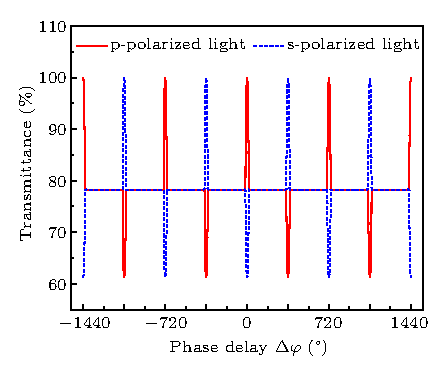
\includegraphics{e1.eps}\\[5pt]  % insert figure
\parbox[c]{15.0cm}{\footnotesize{\bf Fig.~1.}   Transmittance for the eigenvalues of the cavity included
the BP and BC, plotted as a function of $\Delta \varphi $, for the case of
$\beta =45^\circ $.}
\end{center}

\textcolor[rgb]{0.98,0.00,0.00}{$\bullet$ The axis labels should be given in the form of ``variable (unit)''.}

\textcolor[rgb]{0.98,0.00,0.00}{$\bullet$ For single-column figures, the figure width should be smaller than 7.5~cm.}

\newpage
\textbf{Example 2}

\begin{center}
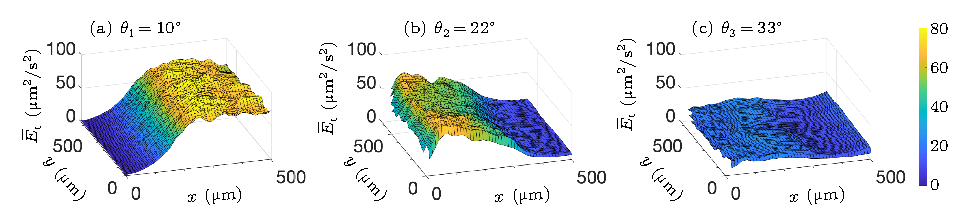
\includegraphics{e2.eps}\\[8pt]
\parbox[c]{15.0cm}{\footnotesize{\bf Fig.~2.}   % figure caption
 Distribution of turbulent kinetic energy. (a)--(c) Corresponding distributions of turbulent kinetic energy averaged over 5000 frames (100~sec) under three confinements. The color shows the intensity of turbulent kinetic energy $\overline{E}_{\rm t}$. Meanwhile, $x=0$~$\rm \upmu m$ indicates the position of the drop contact line.}
\end{center}

\textcolor[rgb]{0.98,0.00,0.00}{$\bullet$ For multi-part figures, different parts must be labeled as (a), (b), (c), etc.}

\textcolor[rgb]{0.98,0.00,0.00}{$\bullet$ Every part should be described in the caption.}

\textcolor[rgb]{0.98,0.00,0.00}{$\bullet$ For double-column figures, the figure width should be smaller than 15~cm.}

\subsection*{4. Table}

Tables are inserted in the center environment.

\textbf{Example 1}

\begin{center}
{\footnotesize{\bf Table 1.} Simulation parameters.\\
\vspace{2mm}
\begin{tabular}{ccc}
\hline
{Variable}      & {Parameter}                         & {Simulation value} \\\hline
{$L$}           & {grating length}                    & {15~mm} \\
{$\varLambda$}  & {grating period}                    & {525.878~nm} \\
{$\lambda_0$}   & {central wavelength}                & {1545.1~nm} \\
{$n_{\rm eff}$} & {effective refractive index}        & 1.4774 \\
{$\delta_n$}    & {refractive index modulation depth} & {$0.9\times 10^{-4}$} \\
\hline
\end{tabular}}
\end{center}

\textbf{Example 2}

\begin{center}
{\footnotesize{\bf Table 2.} Results of the average MSE.\\
\vspace{2mm}
\begin{tabular}{cccccccc}
\hline
&$r_c$ (\AA) &$r_0$ (\AA) &$\kappa r_0$&
&$r_c$ (\AA) &$r_0$ (\AA) &$\kappa r_0$\\
\hline
Cu& 0.800 & 14.10 & 2.550 &Sn$^{\rm a)}$
& 0.680 & 1.870 & 3.700 \\
Ag& 0.990 & 15.90 & 2.710 &Pb$^{\rm b)}$
& 0.450 & 1.930 & 3.760 \\
Au& 1.150 & 15.90 & 2.710 &Ca$^{\rm c)}$
& 0.750 & 2.170 & 3.560 \\
Mg& 0.490 & 17.60 & 3.200 &Sr$^{\rm a)}$
& 0.900 & 2.370 & 3.720 \\
Zn& 0.300 & 15.20 & 2.970 &Li$^{\rm b)}$
& 0.380 & 1.730 & 2.830 \\
Cd& 0.530 & 17.10 & 3.160 &Na$^{\rm c)}$
& 0.760 & 2.110 & 3.120 \\
Hg& 0.550 & 17.80 & 3.220 &K$^{\rm a)}$
&  1.120 & 2.620 & 3.480 \\
Al& 0.230 & 15.80 & 3.240 &Rb$^{\rm b)}$
& 1.330 & 2.800 & 3.590 \\
Ga& 0.310 & 16.70 & 3.330 &Cs$^{\rm c)}$
& 1.420 & 3.030 & 3.740 \\
In& 0.460 & 18.40 & 3.500 &Ba$^{\rm a)}$
& 0.960 & 2.460 & 3.780 \\
Tl& 0.480 & 18.90 & 3.550 & & & & \\
\hline
$^{\rm a)}${Ref.~\cite{2}}, &
$^{\rm b)}${Ref.~\cite{3}}, &
$^{\rm c)}${Ref.~\cite{4}}.
\end{tabular}}
\end{center}


\subsection*{5. References}

\textcolor[rgb]{0.98,0.00,0.00}{$\bullet$ Only published or accepted manuscripts should be included in this reference list;}

\textcolor[rgb]{0.98,0.00,0.00}{$\bullet$ References should all be cited in the main text by using command ucite (Chinese Physics B\ucite{1}) or cite (in Refs.~\cite{1,2,3,4});}

\textcolor[rgb]{0.98,0.00,0.00}{$\bullet$ Each reference item should contain one and only one publication;}

\textcolor[rgb]{0.98,0.00,0.00}{$\bullet$ References must be numbered in the order that they appear in the main text;}

\textcolor[rgb]{0.98,0.00,0.00}{$\bullet$ All authors of a publication should be listed, omission is not allowed unless there are more than 20 of them; \emph{et al.} should be used in the later case after the 3rd author to omit the others.}

Some reference examples are shown below.

\subsubsection*{Journal}

[1] Shahverdiev E M and Shore K A 2005 \emph{Phys. Rev. E } \textbf{71} 016201

[2] Wang J S, Feng J and Zhan M S 2010 \emph{Acta Phys. Sin.} \textbf{50} 299 (in Chinese)

\subsubsection*{Book}

[3] Murrell J N, Carter S, Farantos S C, Huxley P and Varandas A J C 1984 \emph{Molecular
Potential Energy Functions} (Chichester: John Wiley and Sons) p.~9

[4] Bloembergen N 1965 \emph{Nonlinear Optics}, 2nd edn. (New York: Benjamin) pp.~12--15

\subsubsection*{Conference publication}

[5] Tabbal A M, Merel P and Chaker M 1999 \emph{Proceedings of the {\rm 14}th International
Symposium on Plasma Chemistry}, August 2--6, 1999, Prague, Czech Republic, p.~1099

[6] Magen N, Kolodny A, Weiser U and Shamir N 2004 \emph{Proceedings of the International
Workshop on System Level Interconnect Prediction}, February 14--16, 2004, Paris, France, p.~7

\subsubsection*{arXiv}

[7] Latham T and Gershon T 2008 arXiv:0809.0872v1 [hep-ph]

\subsubsection*{Patent}

[8] Plank C J (U.S. Patent) 4 081 490 [1978-02-15]

\subsubsection*{Dissertation}

[9] Guo Z Y 2005 \emph{Optical Readout Infrared Imaging System at Room Temperature} (Ph.D. Dissertation) (Hefei: University of Science and Technology of China) (in Chinese)

\end{CJK*}  %% end the Chinese environment
\end{document}  %%% end document 